\documentclass[a4paper,12pt]{report}
\usepackage[T2A]{fontenc}
\usepackage[utf8]{inputenc}
\usepackage[english,russian]{babel}
\usepackage{graphicx}
\usepackage{wrapfig}
\usepackage{mathtext} 				% русские буквы в фомулах
\usepackage{amsmath,amsfonts,amssymb,amsthm,mathtools} % AMS
\usepackage{icomma} % "Умная" запятая: $0,2$ --- число, $0, 2$ --- перечисление
\usepackage{capt-of}
\usepackage{appendix}
\usepackage{multirow}
\usepackage{hyperref}
\usepackage{floatrow}
\usepackage[left=2cm,right=2cm,
    top=2cm,bottom=2cm,bindingoffset=0cm]{geometry}
\usepackage{multicol} % Несколько колонок
\usepackage{gensymb}
\title{Отчёт по лабораторной работе № 5.5.1. 

Измерение коэффициента ослабления потока $\gamma$-лучей в веществе и определение их энергии.}
\author{Плюскова Н.А. Б04-004 }
\date{\today}
\begin{document}
\maketitle
\section*{1. Аннотация}
В работе будет исследовано ослабление потоков $\gamma$-квантов в железе, свинце и алюминии. Мы найдем коэффициент ослабления потоков и среднюю энергию $\gamma$-лучей, испускаемых источником.

\section*{2. Теоретические сведения}
	Гамма-лучи возникают при переходе возбужденных ядер из одного энергетического состояния в другое, более низкое. Энергия $ \gamma $-квантов обычно заключена между несколькими десятками килоэлектронвольт и несколькими миллионами электрон-вольт. Гамма-кванты не несут электрического заряда, их масса равна нулю. Проходя через вещество, пучок $ \gamma $-квантов постепенно ослабляется. Ослабление происходит по экспоненциальному закону, который может быть записан в двух эквивалентных нормах:
	
	\begin{equation}\label{I(mu)}
	I = I_0 e^{-\mu l}, \quad I_o e^{-\mu 'm_1} 
	\end{equation}
	
	В этих формулах $ I, I_0 $ --- интенсивности прошедшего и падающего излучений, $ l $ --- длина пути, пройденного пучком $\gamma$-лучей, $ m_1 $ --- масса пройденного вещества, приходящаяся на единицу площади, $ \mu $ и $ \mu' $ --- константы, величина которых зависит от вещества, сквозь которое проходят ;$\gamma$-лучи. Длину пути $ l $ обычно выражают в сантиметрах, поэтому $ \mu $ имеет размерность см$ ^{-1} $; величину $ m_1 $ измеряют в г/см$ ^2 $, так что размерность $ \mu' $ равна см$ ^2 $/г. Форма записи через массу является предпочтительной, потому что $ \mu' $, в отличие от $ \mu $, не зависит от плотности среды. 
	
	Ослабление потока $\gamma$-лучей, происходящее при прохождении среды, связано с тремя эффектами: \textbf{фотоэлектрическим поглощением}, \textbf{комптоновским рассеянием} и с \textbf{генерацией электрон-позитронных пар}. Рассмотрим эти эффекты.
	\subsection*{Фотоэлектрическое поглощение.} При столкновении $\gamma$-квантов с электронами внутренних атомных оболочек может происходить поглощение квантов. Энергия $\gamma$-кванта передается соответствующему электрону, а импульс делится между этим электроном и оставшимся после его вылета ионом. Свободный электрон не может поглотить $\gamma$-квант, так как при этом невозможно одновременно удовлетворить законам сохранения энергии и импульса. Наружные электроны не принимают участия в фотоэлектрическом поглощении, потому что они слабо связаны в атоме, так что их практически можно считать свободными. Вероятность $ dP_{\text{ф}} $ фотоэлектрического поглощения $\gamma$-квантов пропорциональна длине пути $ dl $ и плотности электронов в среде (в расчет должны приниматься только электроны, принадлежащие внутренним оболочкам атомов):
	
	\begin{equation}\label{mu ph}
	dP_{\text{ф}} = \sigma_{\text{ф}} n_1 dl, \quad \mu_{\text{ф}} = \sigma_{\text{ф}} n_1
	\end{equation}
	
	Здесь $ n_1 $ --- плотность внутренних электронов, а $ \sigma_{\text{ф}} $ --- поперечное сечение фотоэлектрического поглощения. Поперечное сечение характеризует вероятность фотоэффекта, рассчитанную на один электрон. Связь между $ \mu_{\text{ф}} $ и $ \sigma_{\text{ф}} $ устанавливается из формулы \eqref{I(mu)} и в явном виде определяет зависимости $ \mu $ от плотности среды.
	
	Пусть в результате фотоэффекта энергия $\gamma$-кванта передается
	электрону, находящемуся на $ i $-й оболочке атома. Обозначим через $ W_i $
	энергию связи этого электрона. После вылета из атома электрон приобретает кинетическую энергию $ T_i = \hbar \omega - W_i $.
	Освободившееся после вылета электрона место заполняется затем
	одним из электронов с вышележащих оболочек. При таких переходах
	возникает характеристическое рентгеновское излучение.
	
	\begin{figure}[H]
    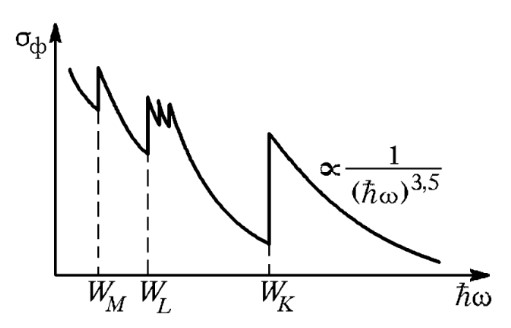
\includegraphics[width = 0.5\textwidth]{2.jpg}
    \centering
    \caption{Зависимость сечения фотоэффекта от энергии $\gamma$-квантов }
    \end{figure}
	
	
	Вероятность фотоэффекта сложным образом зависит от энергии
	$\gamma$-лучей и от заряда ядер. Для оценок можно пользоваться формулой
	
	\begin{equation}\label{sigma ph}
	\sigma_{\text{ф}} \propto \dfrac{Z^5}{(\hbar\omega)^{3,5}}
	\end{equation}
	
	Из формулы \eqref{sigma ph} видно, что вероятность фотоэффекта быстро возрастает при переходе от легких элементов к тяжелым резко падает с увеличением энергии $\gamma$-квантов. На рис. \ref{ris photo} показана энергетическая зависимость сечения фотоэффекта. Из рисунка видно, что при энергиях $\gamma$-квантов, лежащих в области атомных энергий связи, сечение претерпевает резкие изменения: при возрастании энергии это сечение скачкообразно возрастает, когда становится возможным выбивание электронов с очередной оболочки (на рис. \ref{ris photo} это скачки при энергиях $ W_M, W_L, W_K, $ соответствующих энергиям связи $ M, L $  и $ K $-электронов). В этой области сечение фотоэффекта очень велико по сравнению с сечениями других процессов. Поэтому фотоэффект является доминирующим механизмом поглощения $\gamma$-квантов при не очень высоких энергиях.
	
	\subsection*{Комптоновское рассеяние.} Комптоновским рассеянием (или комптоновским эффектом) называется упругое столкновение $\gamma$-кванта с электроном. При таком столкновении $\gamma$-квант передает электрону часть своей энергии, величина которой определяется углом рассеяния. В отличие от фотоэффекта, который может идти только на сильно связанных электронах, комптоновское рассеяние происходит на свободных или слабосвязанных электронах. Роль эффекта Комптона становится
	существенной только тогда, когда энергия квантов становится много
	больше энергии связи электронов в атоме (когда достаточно падает
	вероятность фотоэффекта). Атомные электроны в этом случае можно
	считать практически свободными, что обычно и делается при теоретическом анализе.
	
	Вероятность комптон-эффекта сложным образом зависит от энергии $\gamma$-квантов. В том случае, когда энергия
	$\gamma$-кванта много больше энергии покоя электрона, формула сильно
	упрощается, и выражение для сечения комптон-эффекта приобретает  вид:
	
	\begin{equation}\label{sigma k}
	\sigma_{\text{к}} = \pi r^2 \dfrac{mc^2}{\hbar\omega} \left( \ln{\dfrac{2\hbar\omega}{mc^2} + \dfrac{1}{2}} \right) 
	\end{equation}
	
	где $ r \simeq 2,8 \cdot 10^{13} $ --- классический радиус электрона,$ m $ --- его масса. Из формулы \eqref{sigma k} следует, что сечение комптон-эффекта с ростом энергии фотонов падает далеко не так резко, как сечение фотоэффекта.
	Сечение $ \sigma_{\text{к}} $ относится к одному свободному электрону, в то время как приведенное выше сечение фотоэффекта \eqref{sigma ph} рассчитано на атом.
	Комптоновское рассеяние, отнесенное к атому, оказывается, естественно, в $ Z $ раз больше. 
	
	Комптоновский коэффициент линейного ослабления $ \mu_{\text{к}} $ связан с
	сечением $ \sigma_{\text{к}} $ формулой, аналогичной \eqref{mu ph}. Под $ n $ следует в этом случае понимать плотность слабо связанных электронов, т. е. практически полную плотность электронов в веществе.
	Отметим в заключение, что, в отличие от фотоэффекта, эффект
	Комптона приводит не к поглощению $\gamma$-квантов, а к их рассеянию и
	уменьшению их энергии.
	
	\subsection*{Образование пар}
	
	 При энергиях $\gamma$-лучей, превышающих $ 2mc^2 = 1,02  $МэВ, становится возможен процесс поглощения $\gamma$-лучей, связанный с образованием электрон-позитронных пар. Рождение пар не
	может происходить в вакууме, оно возникает в электрическом поле
	ядер. Вероятность этого процесса приблизительно пропорциональна
	$ Z^2  $ и сложным образом зависит от энергии фотона. При энергиях больше $ 2mc^2  $ фотоэффект даже для самых тяжелых ядер уже не играет
	практически никакой роли. Вероятность образования пар должна поэтому сравниваться с вероятностью комптоновского рассеяния. При
	энергиях, с которыми приходится иметь дело при изучении ядер, рождение пар существенно только в самых тяжелых элементах. Так, даже
	для свинца вероятность рождения пар сравнивается с вероятностью
	комптоновского эффекта только при энергии около 4,7 МэВ.
	\subsection*{Полный коэффициент ослабления $\gamma$-лучей}
	
	Полный линейный коэффициент $ \mu $ ослабления пучка $\gamma$-квантов при прохождении через вещество равен сумме коэффициентов для всех трех рассмотренных процессов. На рис. \ref{ris mu} изображены графики $ \mu $ для различных материалов.
	
	\begin{figure}[h!]
		\centering
		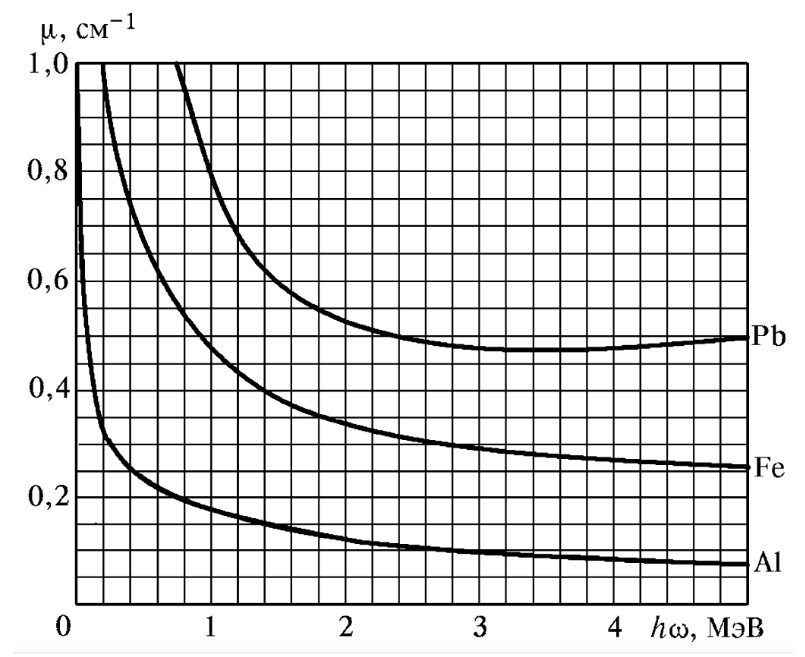
\includegraphics[width=0.6\linewidth]{3.jpg}
		\caption{Полные коэффициенты ослабления потока $\gamma$-лучей в алюминии, железе и свинце}
		\label{ris mu}
	\end{figure}
	
	
	Обратимся вновь к формуле \eqref{I(mu)}. Ее нетрудно получить из теоретических соображений. Рассмотрим опыты, поставленные в хорошей
	геометрии, т. е. в условиях, когда исследуется прохождение сквозь вещество узкого параллельного пучка $\gamma$-лучей. В этом случае не только
	фотоэлектрическое поглощение и генерация пар, но и комптоновское
	рассеяние выводит $\gamma$-кванты из пучка.
	Поэтому при прохождении через вещество меняется только количество, но не энергия $\gamma$-квантов в пучке, так что коэффициент $ \mu $, характеризующий поглощение $\gamma$-квантов в веществе, не зависит от длины
	пути. Обозначим через $ -dN $ число $\gamma$-квантов, выбывших из пучка на
	пути $ dl $. Это число пропорционально имеющемуся их числу $ N $ и пройденному пути $ dl $. Имеем, следовательно,
	
	\begin{equation}\label{N}
	-dN = \mu N dl \Rightarrow N = N_0 e^{-\mu l}
	\end{equation}
	
	т.е то же самое, что и формула \eqref{I(mu)}. В плохой геометрии, когда рассеянные под небольшими углами
	$\gamma$-кванты остаются в пучке, их спектр с прохождением вещества меняется, и формула \eqref{I(mu)}, вообще говоря, неприменима. Эта формула, однако, работает и в этом случае лучше, чем можно было бы ожидать. Причина хорошего согласия заключается в том, что $\gamma$-кванты с энергией 1 -- 2 МэВ, потерявшие энергию из-за комптоновского рассеяния,
	быстро выбывают из пучка из-за резкого увеличения сечений $ \sigma_{\text{ф}} $ и $ \sigma_{\text{к}} $.
	
	В данной работе коэффициент ослабления $ \mu $ измеряется в хорошей
	геометрии. Из формулы \eqref{I(mu)} или \eqref{N} имеем
	
	\begin{equation}\label{mu}
	\mu = \dfrac{1}{l} \ln{\dfrac{N_0}{N}}
	\end{equation}
	
	Для определения коэффициента ослабления нужно, таким образом, измерить толщину образца $ l $, число падающих частиц $ N_0 $ и число
	частиц $ N $, прошедших через образец.

\section*{3. Экспериментальная установка}
\begin{figure}[h!]
		\centering
		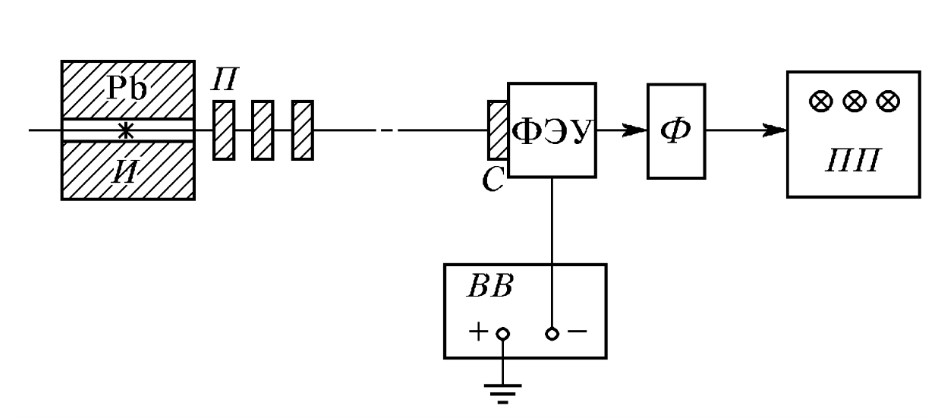
\includegraphics[width=0.7\linewidth]{4.jpg}
		\caption{Блок-схема установки, используемой для измерения коэффициентов ослабления потока $\gamma$-лучей: И --- источник $\gamma$-лучей; $ Pb $ --- свинцовый контейнер с коллиматорным каналом; П --- набор поглотителей; С --- сцинтиллятор (кристалл
			NaI(Tl) ); Ф --- формирователь-выпрямитель}
		\label{ris lab}
	\end{figure}

Схема установки, используемой в работе, показана на рис. \ref{ris lab}. Свинцовый коллиматор выделяет узкий почти параллельный пучок $\gamma$-квантов, проходящий через набор поглотителей П и регистрируемый сцинтилляционным счетчиком). Сигналы от счетчика усиливаются и регистрируются пересчетным прибором ПП. Высоковольтный выпрямитель ВВ обеспечивает питание сцинтилляционного счетчика.

При недостаточно хорошей геометрии в результаты опытов могут
вкрасться существенные погрешности. В реальных установках всегда имеется конечная вероятность того, что $\gamma$-квант провзаимодействует в
поглотителе несколько раз до того, как попадет в детектор. Чтобы уменьшить число таких случаев, в данной работе сцинтилляционный счетчик расположен на большом расстоянии от источника $\gamma$-квантов, а поглотители имеют небольшие размеры. Их следует устанавливать за коллиматорной щелью на некотором расстоянии друг от друга, чтобы испытавшие комптоновское рассеяние и выбывшие из прямого потока кванты с меньшей вероятностью могли в него вернуться.

\section*{4. Ход работы}
\subsection*{4.1 Исследование поглощение $\gamma$-лучей в железе}

После включения пересчетного прибора и высоковольтного выпрямителя, дадим им прогреться в течение 10 минут.

Измерим число частиц $N_{0}$, попадающий в счетчик за фиксированное время $t_{0} = 10$ с в отсутствие поглотителя: $N_{0} = (67062\pm258)$

Измерим число частиц $N$, попадающий в счетчик за фиксированное время в присутствии поглотителя, а также найдем коэффициент ослабления потоков $\gamma$-квантов по формуле 6:

\begin{table}[H]
\begin{tabular}{|c|c|c|c|c|c|c|}
\hline
$t$, с & $N$      & $\sigma_{N}$ & $l$, см & $\sigma_{l}$, см & $\mu$    & $\sigma_{\mu}$ \\ \hline
10   & 35470  & 188          & 1,20  & 0,01             & 0,531 & 0,005    \\ \hline
10   & 38644  & 197          & 2,40  & 0,01             & 0,230 & 0,002    \\ \hline
100  & 109672 & 331          & 3,60  & 0,01             & 0,503 & 0,001    \\ \hline
60   & 37674  & 194          & 4,80  & 0,01             & 0,493 & 0,001    \\ \hline
120  & 45584  & 214          & 6,00  & 0,01             & 0,478 & 0,001    \\ \hline
180  & 40789  & 202          & 7,00  & 0,01             & 0,484 & 0,001    \\ \hline
200  & 27800  & 167          & 8,00  & 0,01             & 0,485 & 0,001    \\ \hline
200  & 17769  & 133          & 9,20  & 0,01             & 0,470 & 0,001    \\ \hline
240  & 14779  & 122          & 10,40 & 0,02             & 0,451 & 0,001    \\ \hline
240  & 10981  & 105          & 11,40 & 0,02             & 0,438 & 0,001    \\ \hline
\end{tabular}
\caption{Число частиц, попадающий в счетчик в присутствии железа}
\end{table}

\begin{equation*}
    \mu_{Fe} \approx (0,481\pm0,005)\text{см}^{-1}
\end{equation*}

Погрешность $\mu$ считали по формуле:
\begin{equation*}
    \sigma_{\mu} = \sqrt{(ln\frac{N_{0}t}{Nt_{0}}\frac{1}{l^{2}}*\sigma_{l})^{2} + (\frac{1}{Nl}*\sigma_{N})^2}
\end{equation*}

\subsection*{4.2 Исследование поглощение $\gamma$-лучей в свинце}

Измерим число частиц $N_{0}$, попадающий в счетчик за фиксированное время $t_{0} = 10$ с в отсутствие поглотителя: $N_{0} = (70452\pm265)$

Измерим число частиц $N$, попадающий в счетчик за фиксированное время в присутствии поглотителя, а также найдем коэффициент ослабления потоков $\gamma$-квантов по формуле 6:

\begin{table}[H]
\begin{tabular}{|c|c|c|c|c|c|c|}
\hline
$t$, с & $N$     & $\sigma_{N}$ & $l$, см & $\sigma_{l}$, см & $\mu$    & $\sigma_{\mu}$ \\ \hline
20   & 73560 & 271          & 0,50  & 0,01             & 1,300 & 0,015    \\ \hline
20   & 44648 & 211          & 0,94  & 0,01             & 1,223 & 0,010    \\ \hline
60   & 77180 & 278          & 1,42  & 0,01             & 1,198 & 0,008    \\ \hline
60   & 48606 & 220          & 1,90  & 0,01             & 1,138 & 0,006    \\ \hline
120  & 66638 & 258          & 2,32  & 0,01             & 1,095 & 0,006    \\ \hline
120  & 43163 & 208          & 2,80  & 0,01             & 1,062 & 0,005    \\ \hline
180  & 42056 & 205          & 3,28  & 0,01             & 1,039 & 0,004    \\ \hline
240  & 39948 & 200          & 3,77  & 0,01             & 0,993 & 0,004    \\ \hline
240  & 29499 & 172          & 4,23  & 0,02             & 0,957 & 0,004    \\ \hline
240  & 25469 & 160          & 4,71  & 0,02             & 0,891 & 0,003    \\ \hline
\end{tabular}
\caption{Число частиц, попадающий в счетчик в присутствии свинца}
\end{table}

\begin{equation*}
    \mu_{Pb} \approx (1,090\pm0,02)\text{см}^{-1}
\end{equation*}

Погрешность $\mu$ считали по формуле:
\begin{equation*}
    \sigma_{\mu} = \sqrt{(ln\frac{N_{0}t}{Nt_{0}}\frac{1}{l^{2}}*\sigma_{l})^{2} + (\frac{1}{Nl}*\sigma_{N})^2}
\end{equation*}


\subsection*{4.3 Исследование поглощение $\gamma$-лучей в алюминии}

Измерим число частиц $N_{0}$, попадающий в счетчик за фиксированное время $t_{0} = 10$ с в отсутствие поглотителя: $N_{0} = (69736\pm264)$

Измерим число частиц $N$, попадающий в счетчик за фиксированное время в присутствии поглотителя, а также найдем коэффициент ослабления потоков $\gamma$-квантов по формуле 6:

\begin{table}[H]
\begin{tabular}{|c|c|c|c|c|c|c|}
\hline
$t$, с & $N$      & $\sigma_{N}$ & $l$, см & $\sigma_{l}$, см & $\mu$    & $\sigma_{\mu}$ \\ \hline
20   & 86890  & 295          & 2,00  & 0,01             & 0,237 & 0,002    \\ \hline
20   & 57131  & 239          & 4,00  & 0,01             & 0,223 & 0,001    \\ \hline
60   & 114297 & 338          & 6,00  & 0,01             & 0,216 & 0,001    \\ \hline
60   & 77062  & 278          & 8,00  & 0,01             & 0,211 & 0,001    \\ \hline
60   & 51670  & 227          & 10,00 & 0,01             & 0,209 & 0,000    \\ \hline
120  & 71386  & 267          & 12,00 & 0,01             & 0,205 & 0,000    \\ \hline
120  & 49694  & 223          & 14,00 & 0,01             & 0,202 & 0,000    \\ \hline
180  & 53635  & 232          & 15,98 & 0,01             & 0,197 & 0,000    \\ \hline
240  & 52454  & 229          & 17,96 & 0,02             & 0,193 & 0,000    \\ \hline
240  & 40352  & 201          & 19,96 & 0,02             & 0,187 & 0,000    \\ \hline
\end{tabular}
\caption{Число частиц, попадающий в счетчик в присутствии алюминия}
\end{table}


\begin{equation*}
    \mu_{Al} \approx (0,208\pm0,02)\text{ см}^{-1}
\end{equation*}

Погрешность $\mu$ считали по формуле:
\begin{equation*}
    \sigma_{\mu} = \sqrt{(ln\frac{N_{0}t}{Nt_{0}}\frac{1}{l^{2}}*\sigma_{l})^{2} + (\frac{1}{Nl}*\sigma_{N})^2}
\end{equation*}


\subsection*{4.4 Измерение шума и дальнейшая обработка результатов}
Измерим фон, обусловленный шумом ФЭУ и посторонними частицами : 

\begin{center}
   $t_{bg} = 300$ с $N_{bg} = (3406\pm58)$ 
\end{center}


Построим график $ln(\frac{N}{t}-\frac{N_{bg}}{t_{bg}})(l)$, по углу наклона которого найдем $\mu^\prime$:

	\begin{figure}[H]
		\centering
		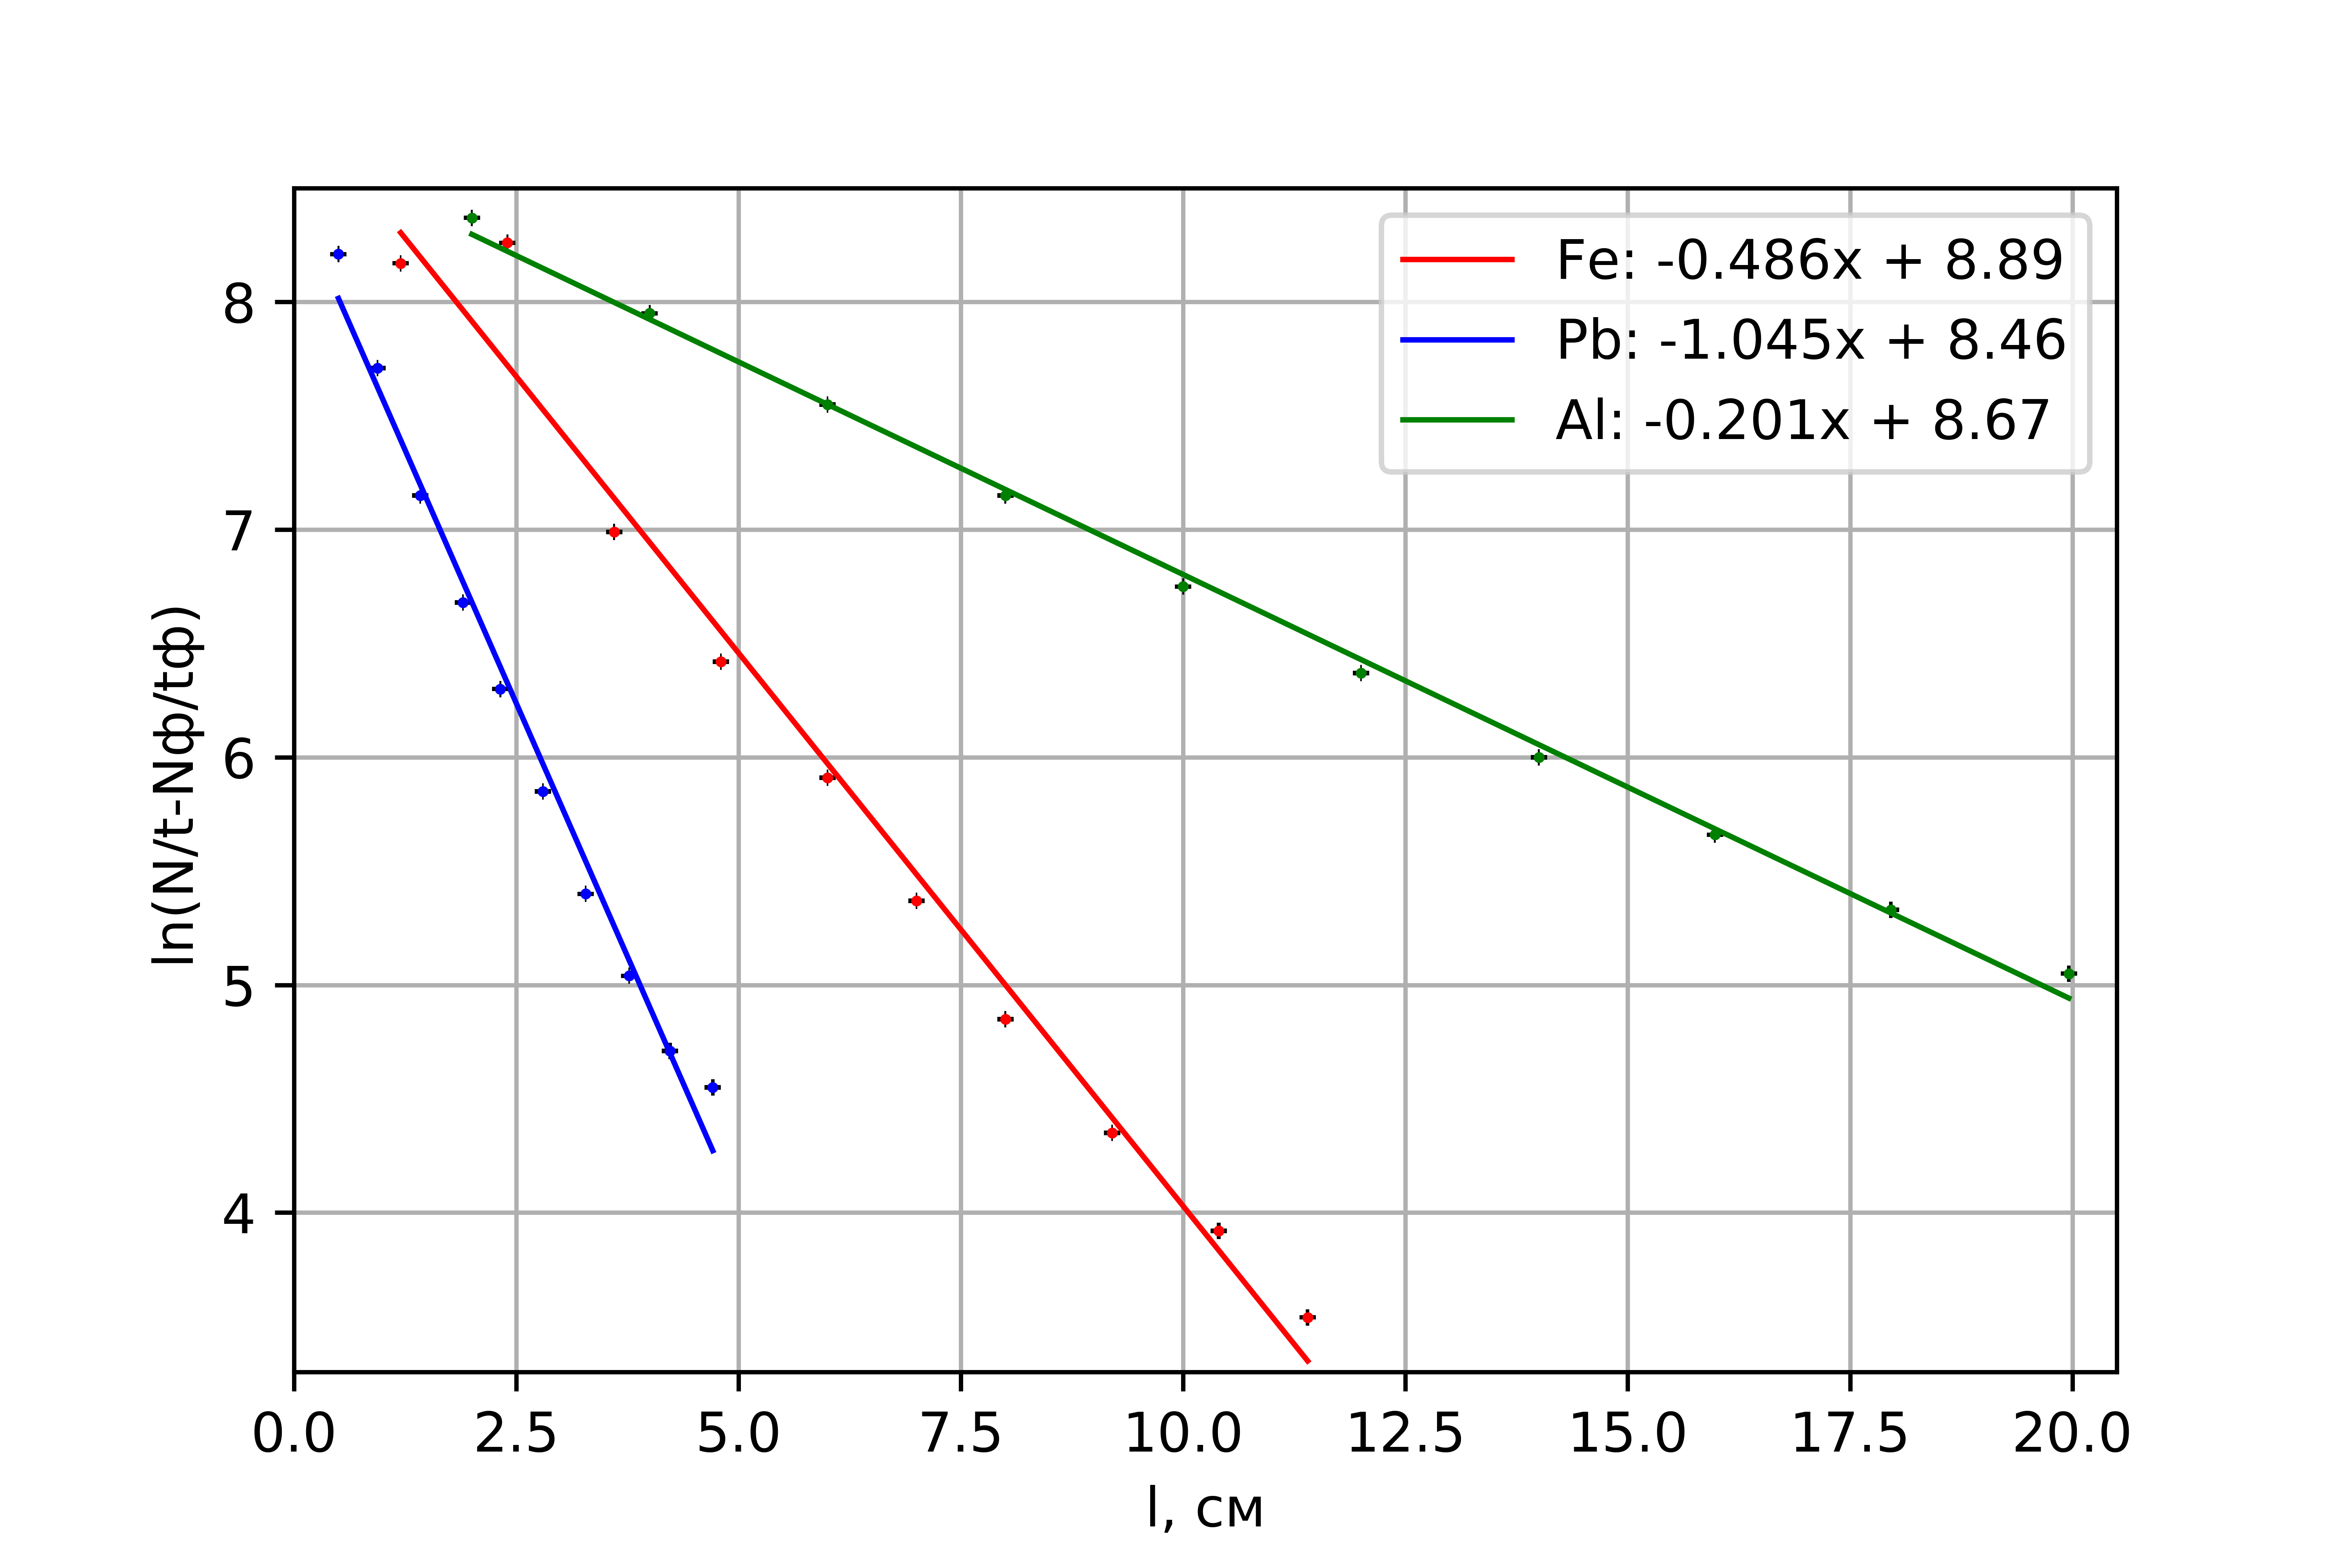
\includegraphics[width=0.8\linewidth]{find_mu.png}
		\caption{$ln(\frac{N}{t}-\frac{N_{bg}}{t_{bg}})(l)$}
		\label{ris mu}
	\end{figure}

\begin{equation*}
\begin{gathered}
    \mu_{Fe} = (0,49\pm 0,01) \text{см}^{-1}; \\
    \mu_{Pb} = (1,03\pm 0,02) \text{см}^{-1}; \\
    \mu_{Al} = (0,19\pm 0,01) \text{см}^{-1};
\end{gathered}
\end{equation*}

Заметим, что найденные значения коэффициента ослабления потоков $\gamma$-квантов сходятся в пределах $3\sigma$

По найденному значению коэффициента ослабления потоков $\gamma$-квантов и известной зависимости $\mu(E)$ для данных металлов найдем среднюю энергию $\gamma$-лучей, испускаемых источником:

	\begin{figure}[H]
		\centering
		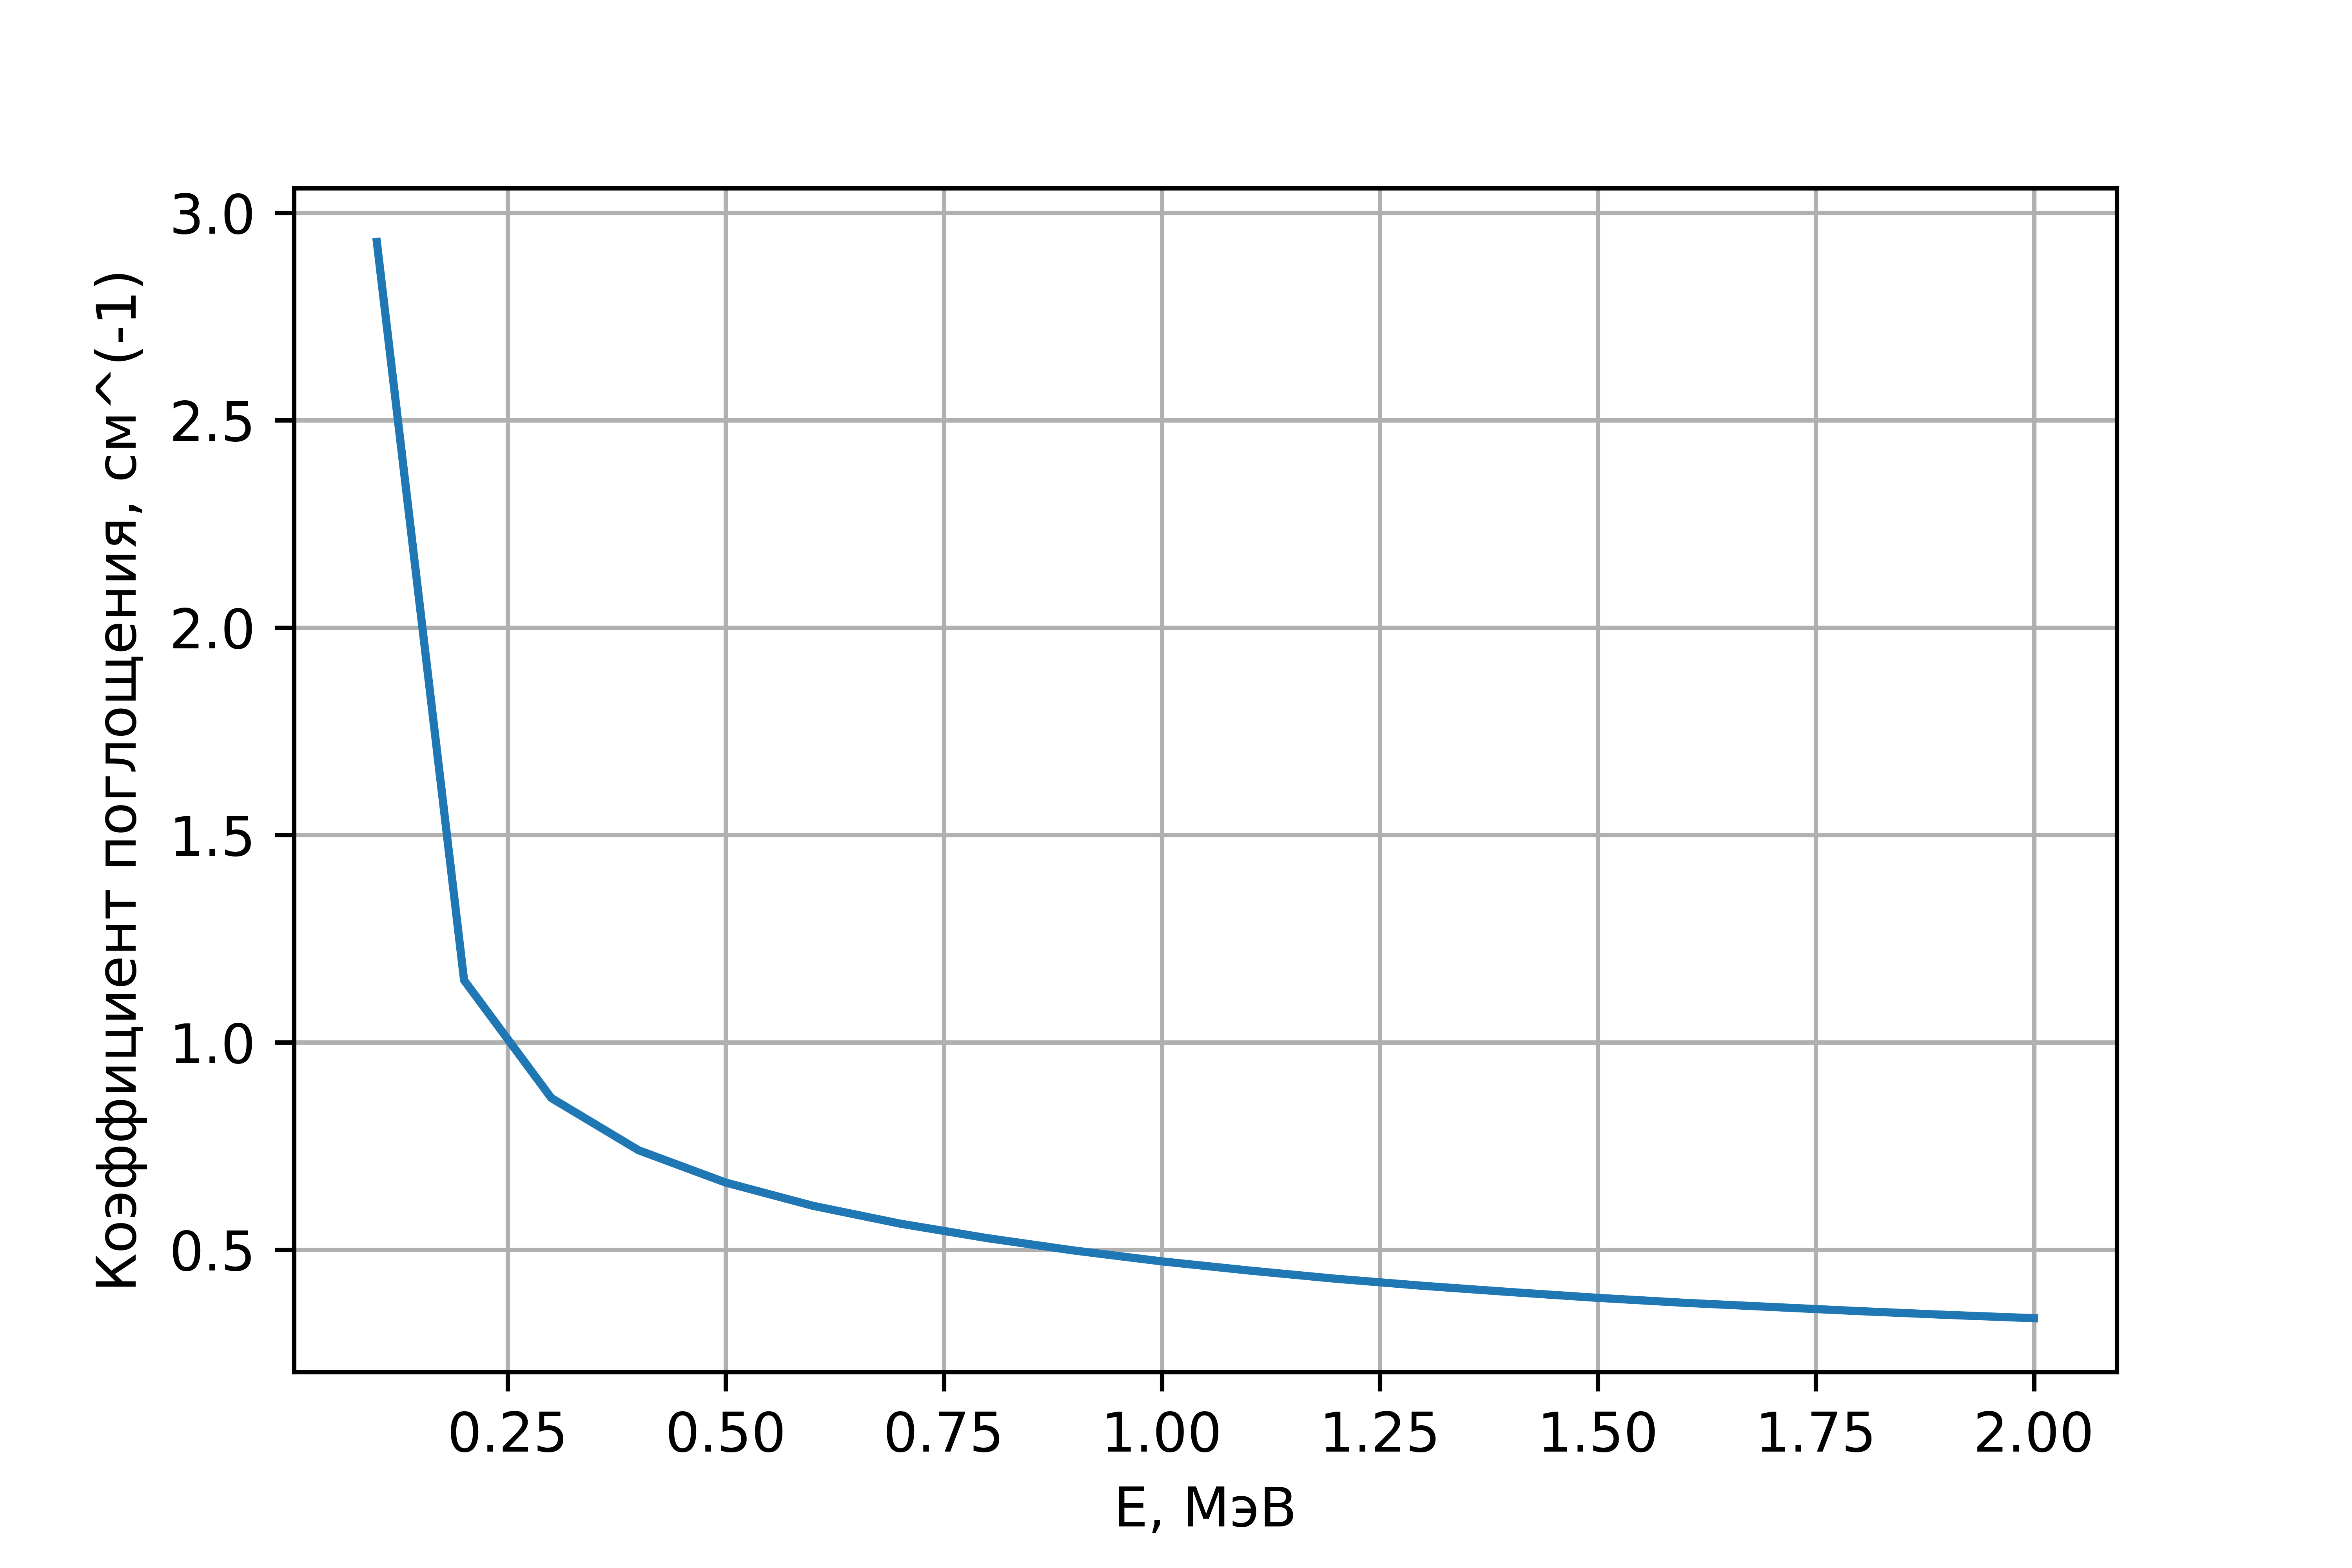
\includegraphics[width=0.8\linewidth]{mu(E)_fe.png}
		\caption{$\mu(E)$ для железа}
		\label{ris mu}
	\end{figure}
	
\begin{equation*}
E_{Fe} = (0,82\pm0,02)\text{ МэВ}
\end{equation*}	
	
	\begin{figure}[H]
		\centering
		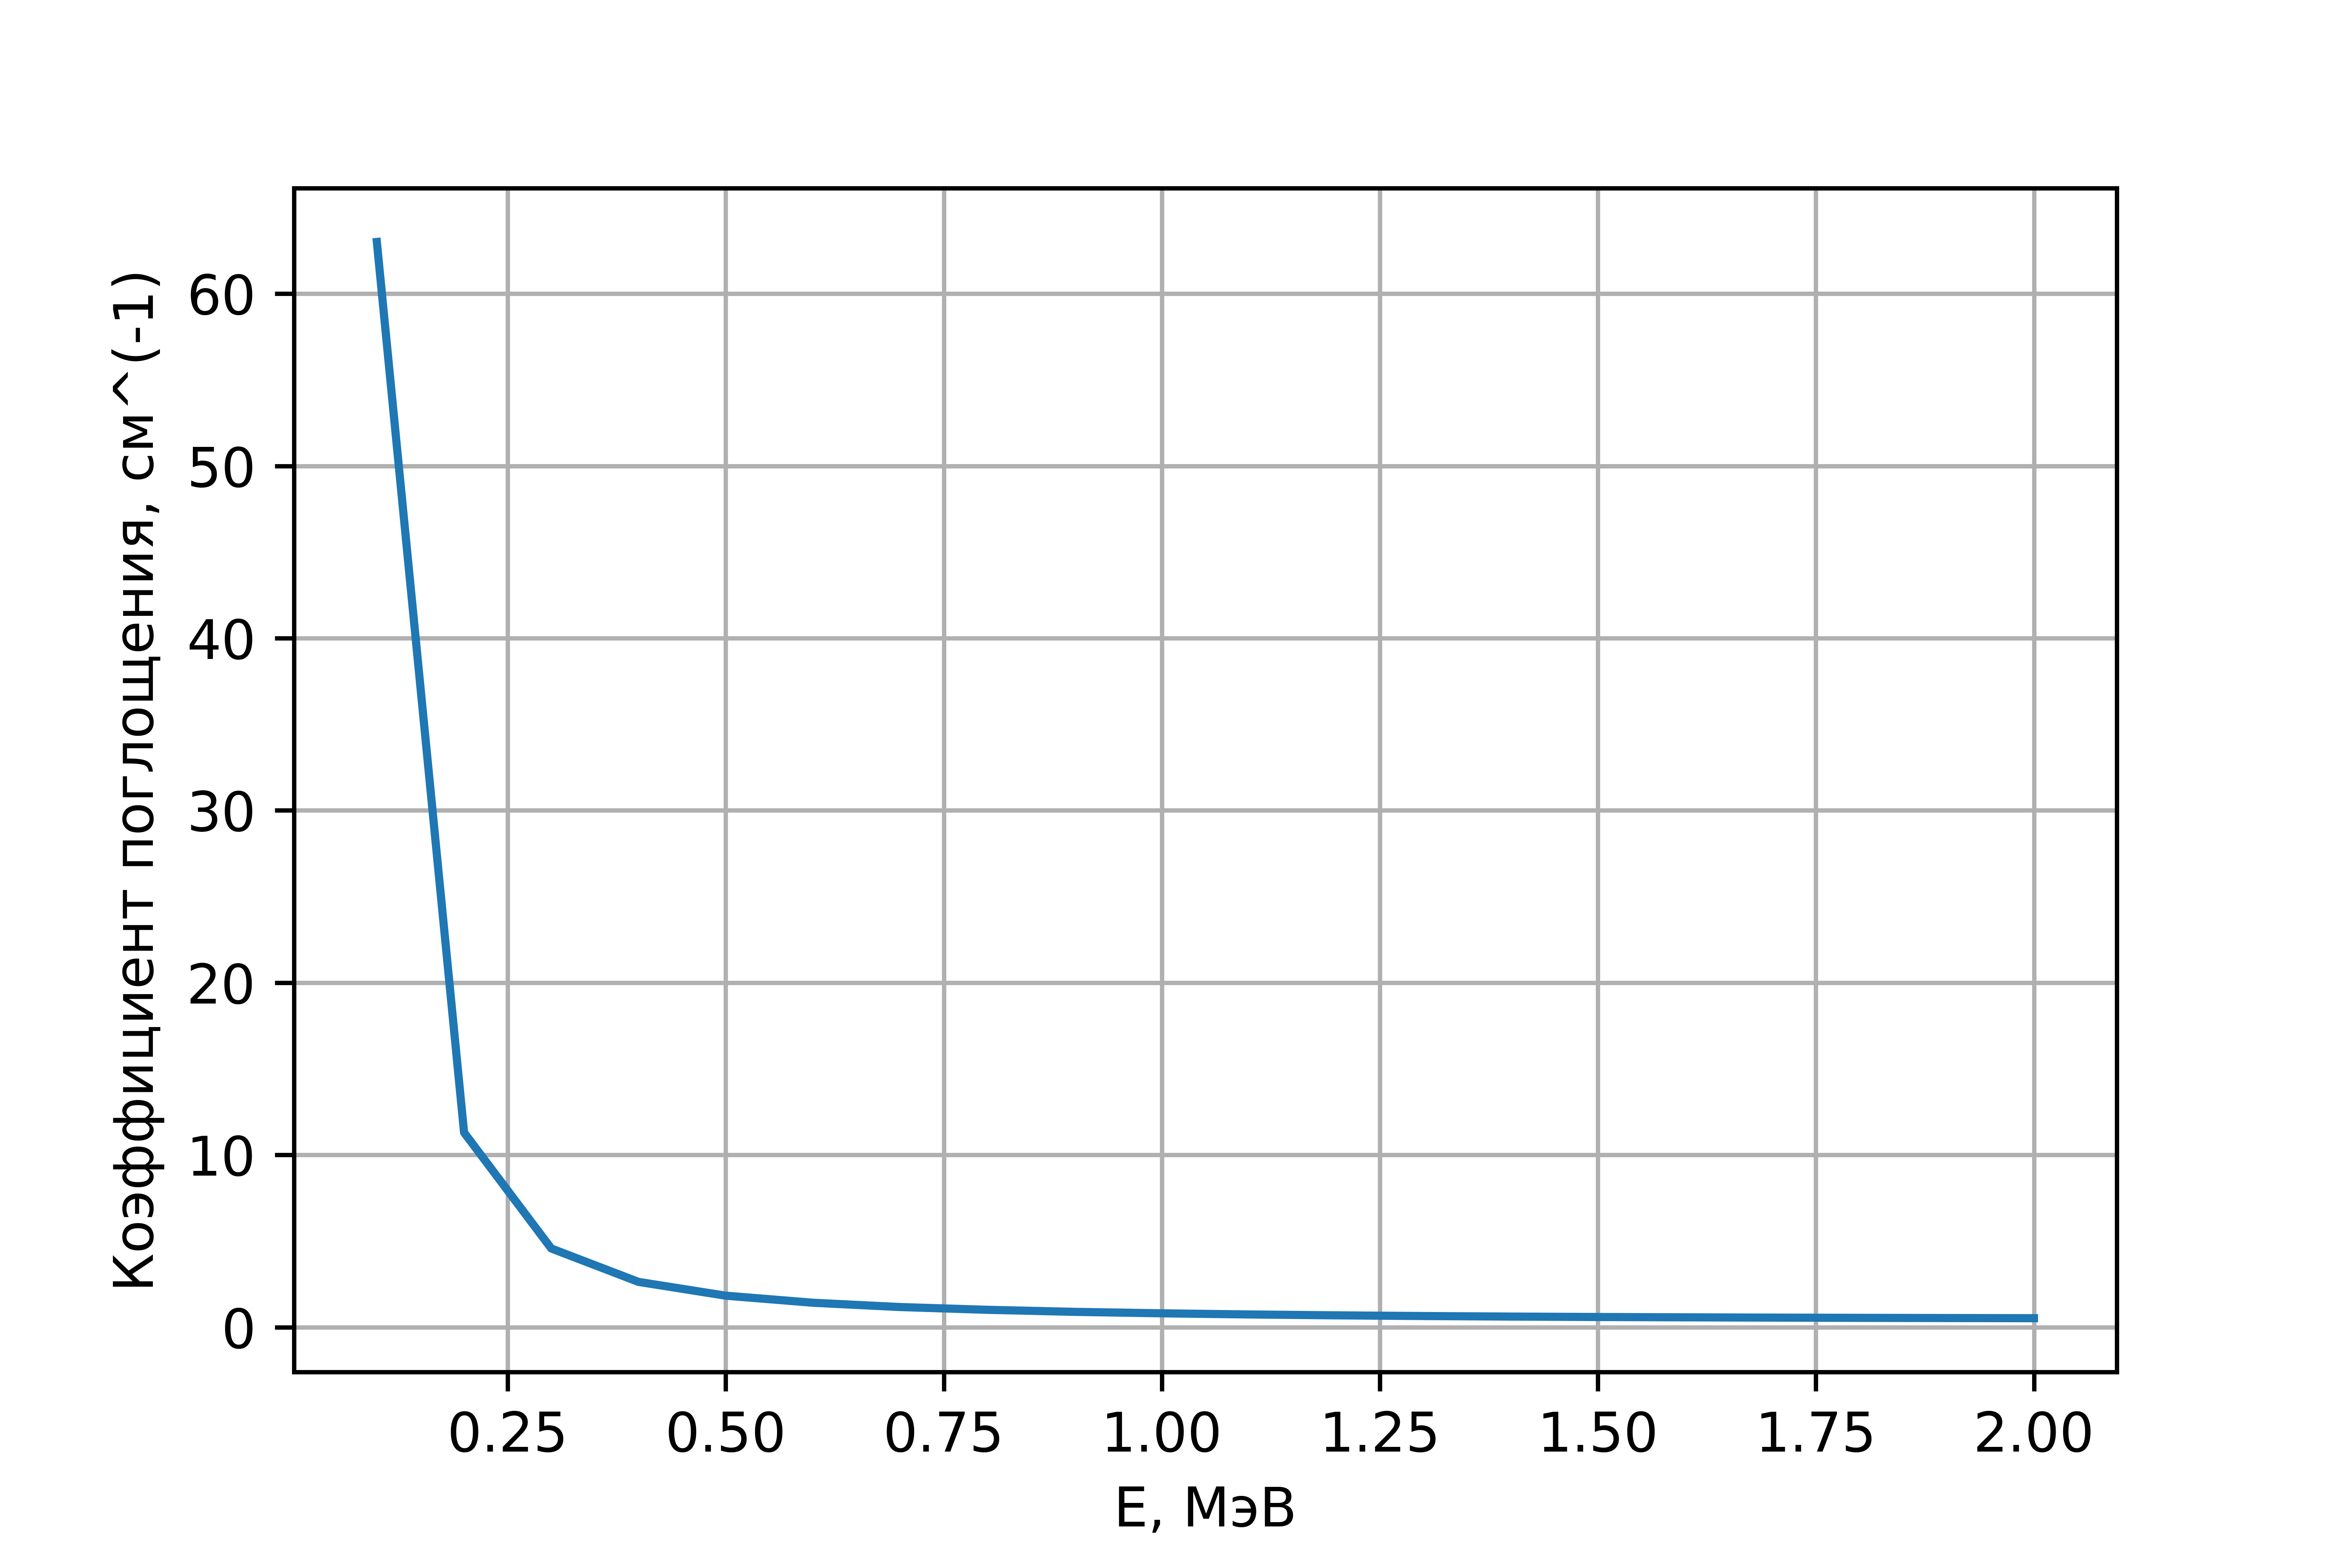
\includegraphics[width=0.8\linewidth]{mu(E)_pb.png}
		\caption{$\mu(E)$ для свинца}
		\label{ris mu}
		
\begin{equation*}
E_{Pb} = (0,78\pm0,02)\text{ МэВ}
\end{equation*}	
		
	\end{figure}
		\begin{figure}[H]
		\centering
		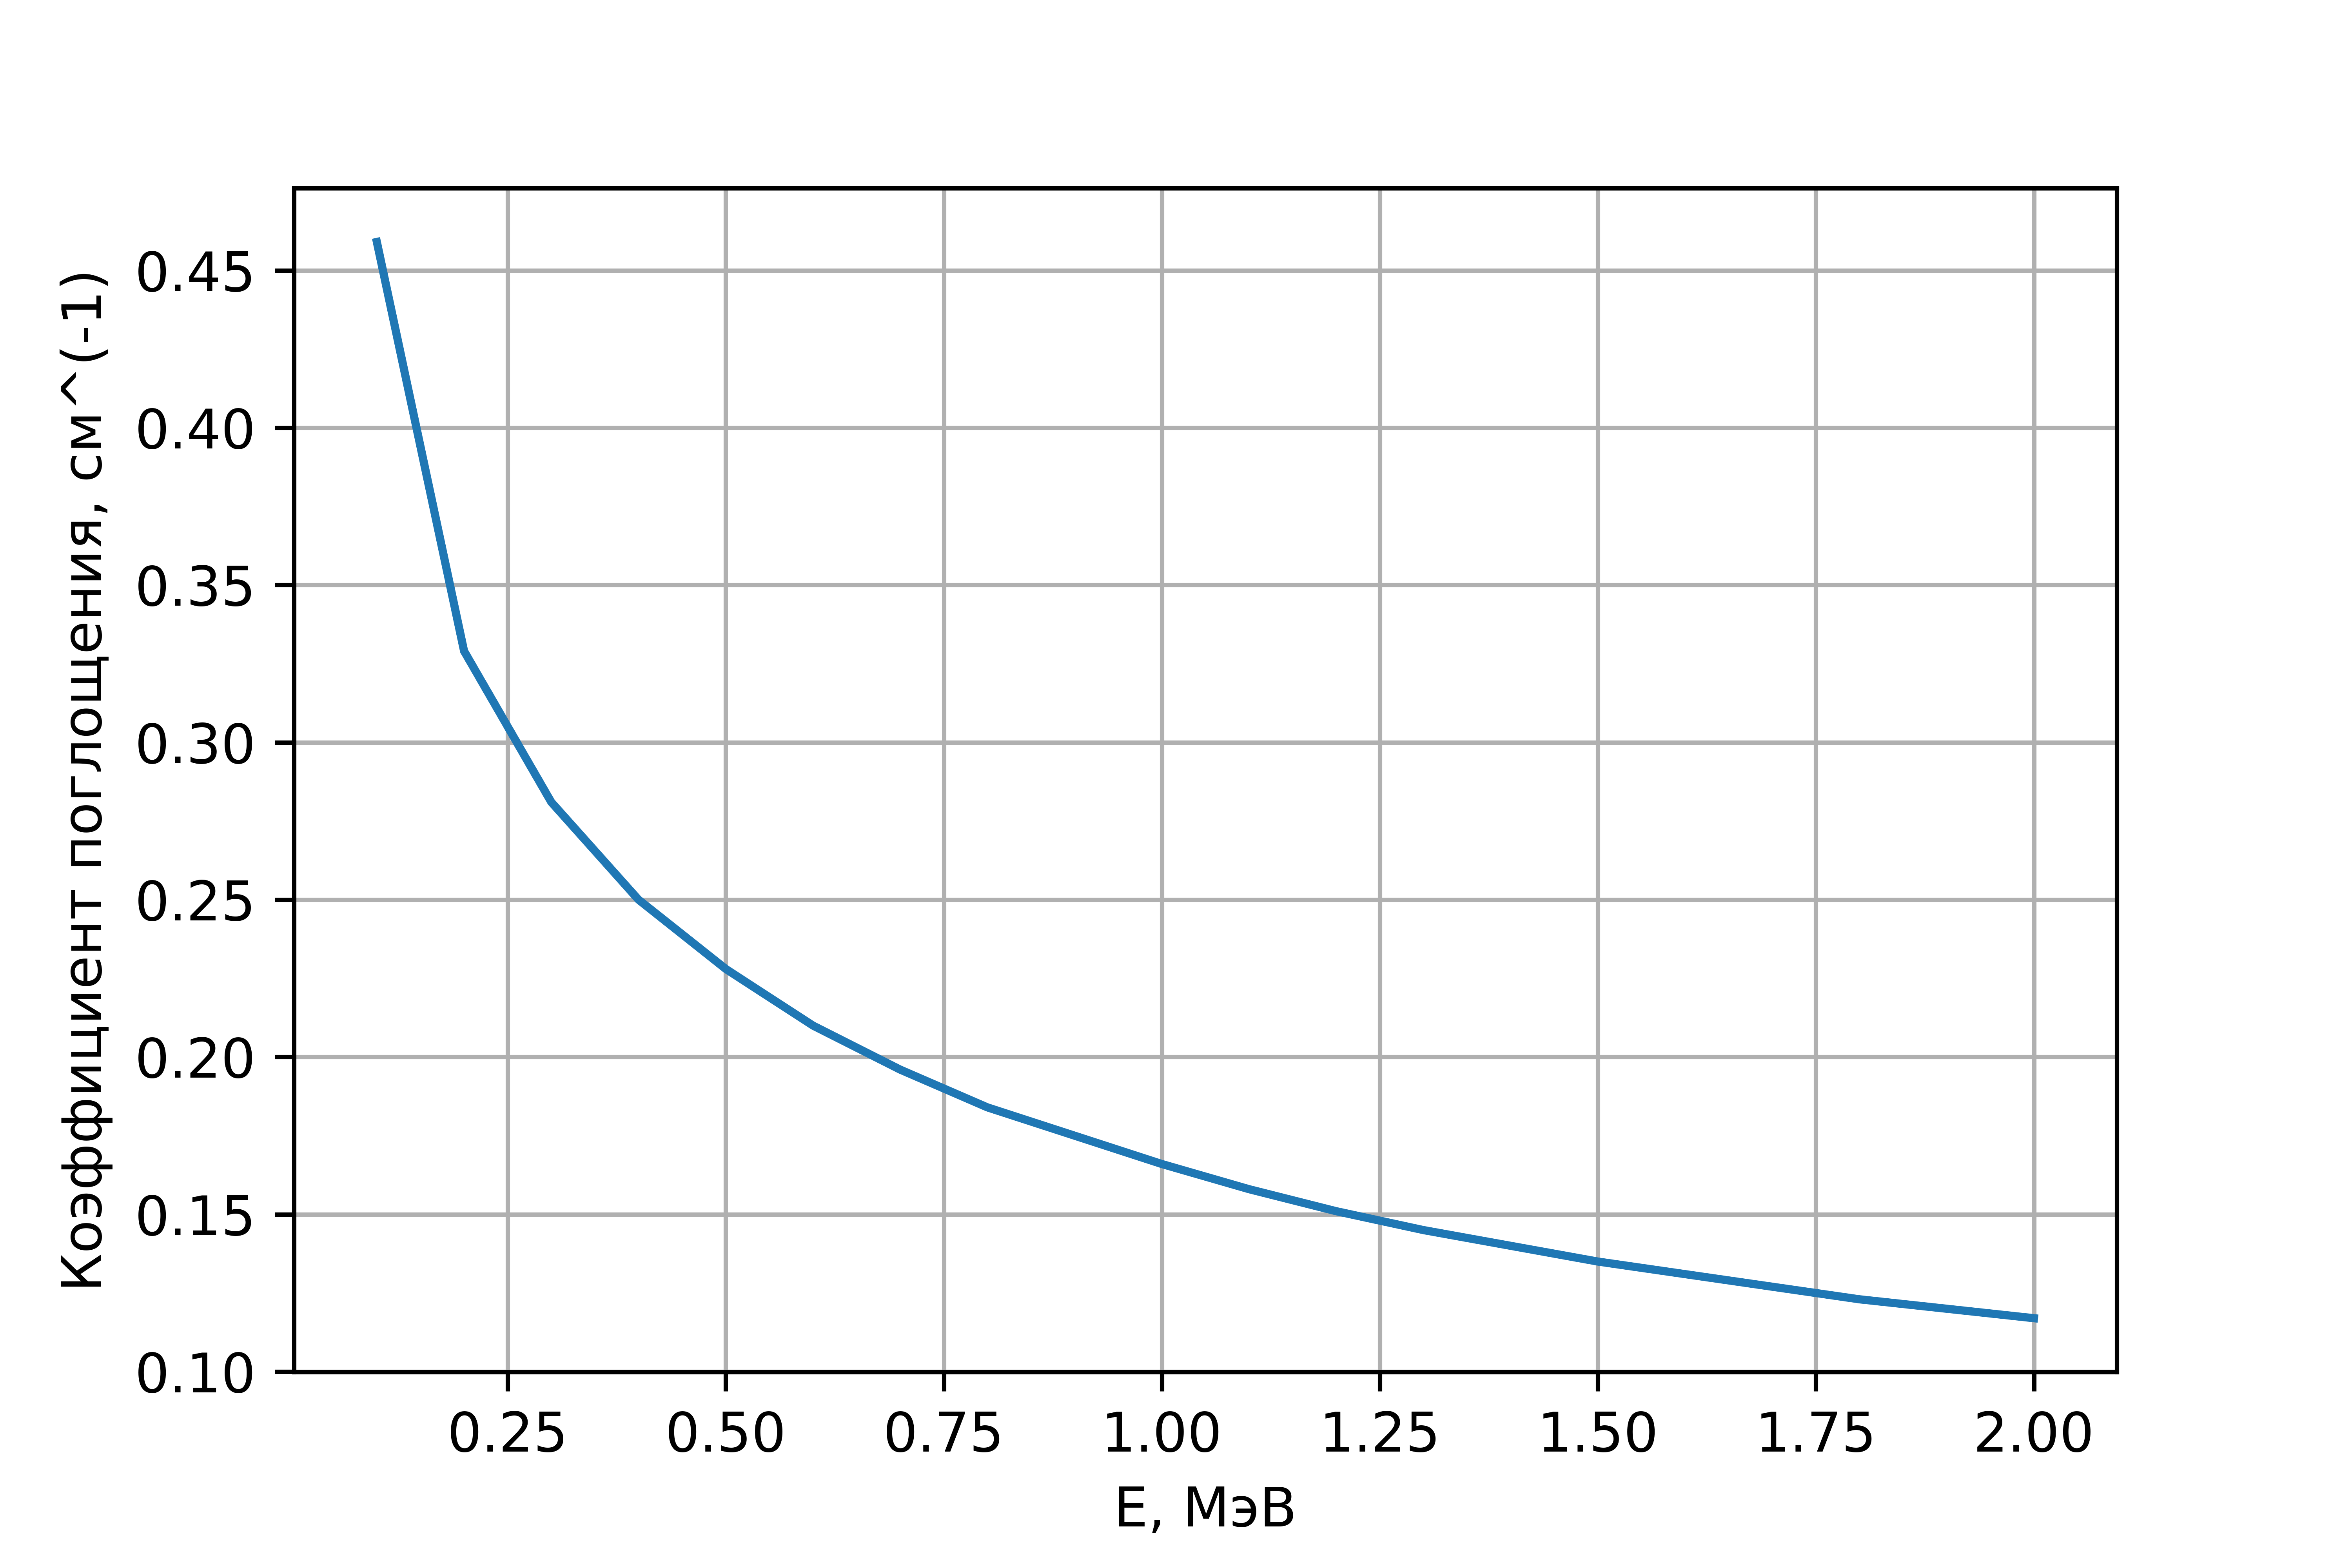
\includegraphics[width=0.8\linewidth]{mu(E)_al.png}
		\caption{$\mu(E)$ для алюминия}
		\label{ris mu}
	\end{figure}
	
\begin{equation*}
E_{Al} = (0,76\pm0,03)\text{МэВ}
\end{equation*}	

\section*{5. Выводы}
Мы исследовали ослабление потоков $\gamma$-квантов в трех веществах: железе, свинце и алюминии. Двумя способами нашли коэффициент ослабления потоков $\gamma$-квантов:
\begin{table}[H]
\begin{tabular}{|c|c|c|}
\hline
         & $\mu_{formula}$, см^{-1}    & $\mu_{graph}$, см^{-1}  \\ \hline
железо   & 0,481 \pm 0,005 & 0,49 \pm 0,01 \\ \hline
свинец   & 1,090 \pm 0,02  & 1,03 \pm 0,02 \\ \hline
алюминий & 0,208 \pm 0,02  & 0,19 \pm 0,01 \\ \hline
\end{tabular}
\end{table}

Заметим, что найденные значения сходятся в пределах $3\sigma$.
Также была получена средняя энергию $\gamma$-лучей, испускаемых источником:
\begin{equation*}
\begin{gathered}
    E_{Fe} = (0,82\pm0,02)\text{ МэВ}; \\
    E_{Pb} = (0,78\pm0,02)\text{ МэВ}; \\
    E_{Al} = (0,76\pm0,03)\text{МэВ};
\end{gathered}
\end{equation*}
	
Получаем, что средняя энергия $\gamma$-лучей источника $E \approx 0,79$МэВ
\end{document}
